
\chapter{用户画像建模}
\label{chap:example}
Alan Cooper(交互设计之父)最早提出了用户画像(persona)的概念:“Personas are a concrete representation of target users”。Persona 是真实用户的虚拟代表,是建立在一系列真实数据(Marketing data,Usability data)之上的目标用户画像。通过用户历史行为去了解用户,根据他们的目标、行为和观点的差异,将他们区分为不同的类型,然后每种类型中抽取出典型特征,赋予名字、照片、一些人口统计学要素、兴趣标签等描述,就形成了一个人物原型(personas),\autoref{pic:hl_userProfile}所示为一个典型的用户画像,标签面积越大代表其权重越高。一些大公司很喜欢用personas做用研究,比如阿里,腾讯,微软等,刻画每个用户,是任何一家社交类型的服务都需要面对的问题,不同的公司针对各自业务会有不同的需求,构建用户画像的动机和目标也会存在一定差异。从手机主题应用商城的角度来讲,构建用户画像的目的包括:

\begin{figure}
\centering
  \framebox{\includegraphics[scale=0.35]{figures/hl_userProfile}}
  \figcaption{用户画像标签化}
  \label{pic:hl_userProfile}
\end{figure}

\begin{itemize}
\item 完善及扩充用户信息。用户画像的首要动机就是了解用户,这样才能够提供更优质的服务。但是在实际中用户的信息提供得不尽完整,有些是因为平台的引导机制造成的,有时候又是用户不愿意或懒得提供,而且对于用户自行输入的内容又很难进行规范化此外,一些隐性或变化频繁的信息也需要通过用户的行为挖掘出来。
\item 打造健康的主题设计生态圈。在掌握用户信息的基础上,平台就可以对自身的状况进行分析,从相对宏观的基础上把握主题市场的生态环境,挖掘设计作品的最大价值,帮助设计师提高收入,\autoref{pic:hl_income}。例如通过对用户信息的聚类,能够对用户进行人群的划分,掌握不同人群的活跃程度、行为及兴趣偏好,热门主题的传播方式和流行引爆点等。
\begin{figure}
\centering
  \framebox{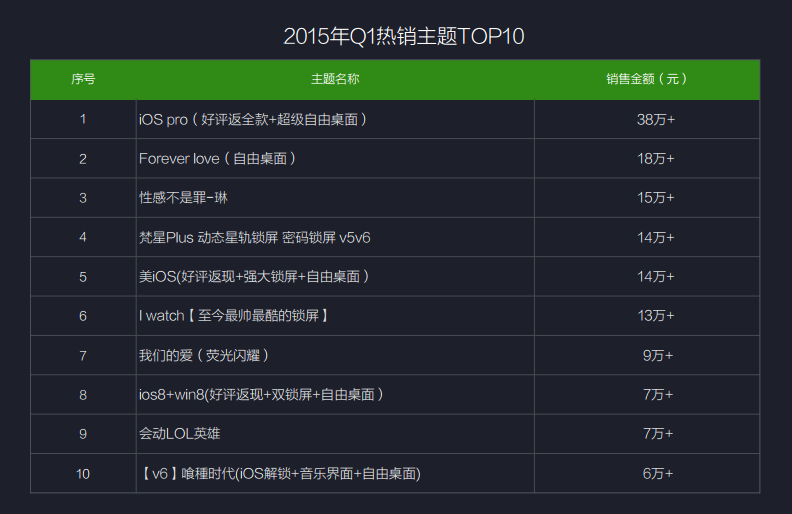
\includegraphics[scale=0.45]{figures/hl_income}}
  \figcaption{2015年Q1热销主题排行榜}
  \label{pic:hl_income}
\end{figure}

\item 支撑主题推荐系统的精准推荐。精准推荐的前提是对用户的清晰认知。以简单代金券发放为例,手机主题应用市场的历史数据呈现出两大类四种不同的消费习惯。代金券敏感型:发代金券才用、发代金券用的更多;代金券不敏感型:发不发都用,发代金券也不用。在推荐系统的用户画像系统中,上述四种群体会被分别冠以屌丝、普通、中产、土豪的标签。针对四类用户的运营策略也会全然不同,最直接的就是代金券的刺激频率以及刺激金额,而对“代金券”免疫的土豪群体,则更多地需要在优化服务上做文章。在实际场景中,影响用户对手机主题包的使用黏度的因素要远比代金券复杂得多,在这种情况下,利用用户画像可以对用户的“贴身跟踪”就能及时发现薄弱环节,因此从用户打开应用商店到退出使用,其间的每一步情况都被快的记录在案:哪一天退出的,哪一步退出的,退出之后“跳转”到什么软件等等。据此,用户画像也实现了用户另外一个纬度的归类,分清哪部分是忠实用户,哪部分可能是潜在的忠实用户,哪些则是已经流失的;更进一步来看流失的原因:因为代金券没有了流失?主题包质量不好流失?这些都是下一步精准推荐的依据。其实手机主题市场中的各项业务都与用户画像有着直接与间接的关系,无论是基于兴趣的推荐提升用户价值,精准的广告投放提升商业价值,还是针对特定用户群体的内容运营,用户画像都是其必不可少的基础支撑。直接地,用户画像可以用于兴趣匹配、关系匹配的推荐和投放;间接地,可以基于用户画像中相似的兴趣、关系及行为模式去推动用户兴趣和设计师的无缝对接。
\item 主题市场安全领域的应用。随着手机主题市场的发展,商家会通过各种活动形式的补贴来获取用户、培养用户的消费习惯,但同时也催生一些通过刷排行榜、刷红包的用户,这些行为距离欺诈只有一步之遥,但他们的存在严重破环了市场的稳定,侵占了活动的资源。其中一个有效的解决方案就是利用用户画像沉淀方法设置促销活动门槛,即通过记录用户的注册时间、历史登陆次数、常用IP地址等,最大程度上隔离掉僵尸账号,保证市场的稳定发展。
\end{itemize}

用户画像的目的是将用户信息标签化,本文介绍针对主题应用商店本身的特点介绍用户画像的构建,该用户画像主要还是从电子商务的角度出发,完善用户信息和发掘用户兴趣,区分兴趣和购买意愿,并形式化、结构化表达出来。数据的来源也主要是主题平台本身,并没有采用更多的第三方数据。

    \section{用户画像的数据来源}
    手机主题用户画像的信息来源可以有如下几种方式:
    \begin{itemize}
    \item 显式用户行为。显式方法主要是通过获取用户注册信息中的有关的兴趣和偏好或允许用户自己定义和修改用户画像来实现,一般获取的是用户相对静态和稳定的属性,例如:性别、年龄区间、地域、受教育程度、学校、公司等。主题应用商店本身就有比较完整的用户注册引导、用户信息完善任务、认证用户审核等,在收集和清洗用户属性的过程中,需要注意的主要是标签的规范化以及不同来源信息的交叉验证。
    \item 隐式用户行为。隐式方法则是通过跟踪用户的行为和交互来评估和推测用户画像,一般获取的是用户更加动态和易变化的兴趣特征,首先,用户兴趣会受到环境、热点事件、季节等方面的影响,一旦这些因素发生变化,用户的兴趣容易产生迁移;其次,用户的行为多样且碎片化,不同行为反映出来的兴趣差异较大。
    \item 第三方应用数据。一些功能性应用如微信、微博提供的第三方免注册登陆API接口,可以直接获取第三方应用账号提供的用户基本数据。
    \item 自然语言处理技术。利用自然语言处理技术提取用户购买评价、评论语句中的关键词,作为用户画像标签的一部分。
    \end{itemize}

    在个性化服务的用户画像建模中,最常用的方式是将以上几种或多种方法结合起来,通过显式方式来获取静态用户信息如姓名、性别、职业等;通过隐式方式来获取动态用户信息如用户兴趣、爱好等;通过第三方登陆接口获取用户的分享、动态信息等;通过自然语言处理技术分析用户的当前心态、满意度、消费心情等。

    \section{标签权重计算}
    推荐本质上是一种个性化排序,因此在收集到一个用户可能存在的标签后,还需要给标签赋一定的权重,用来区分不同标签对于该用户的重要程度。一个标签对于特定用户的权重值可以大致表示为:标签权重 = (行为类型 + 时空上下文 + 长尾因子) × 时间衰减因子。举例,用户小磊昨天购买了一款win8风格的主题包,计算公式如\autoref{tab:tagweight}所示。
    \begin{table}[htp]
    \centering
    \tabcaption{标签权重计算公式}
    \label{tab:tagweight}
    \begin{tabular}{|c|p{8cm}|} \hline
     标签 & win8风格,比较大众化,长尾因子记为 1 \\ \hline
     时间 & 昨天,衰减因子为 0.95。 \\ \hline
     行为 & 购买行为,记为权重 5 \\ \hline
     上下文 & 用户通过关键字搜索进入,最近几天有多次浏览行为,记为权重 2+2 \\ \hline
     标签权重 &  (5+1+4)*0.95=9.5 \\ \hline
    \end{tabular}
    \end{table}

    其中,用户行为类型一般有浏览、添加购物车、搜索、评论、购买、点击赞、收藏等,不同的行为类型具有不同的权重,如购买权重计为5,浏览计为1。空间上下文是指用户跳转入口方式,如通过搜索入口权重高一些,排行榜入口低一些,时间上下文是指用户之前是否接触过此类标签,接触频率等。长尾因子是指,如果标签本身是一个非常常见的词,那么它用于刻画用户的兴趣的区分性是比较差的,相反如果是一个长尾词,则区分性较强。出于这样的考虑,越是长尾词,标签的权重值会越高。标签的权重也随着时间的流逝而变化,用户的兴趣会发生转移,时间越久远,标签的权重应该相应的下降,距离当前时间越近的兴趣标签应该得到适当突出。出于这样的考虑,一般会在标签权重值上叠加一个时间衰减函数并体现不同的时效性。此外,针对用户的兴趣,还会设定一个较小的时间窗口来获取用户的短期兴趣,短期兴趣更新周期会较长期兴趣更短,兴趣更集中,但是能够比较及时地反应用户兴趣的变化。实际生产中标签权重计算需要人工参与调整,流程如\autoref{pic:hl_abtest}
    \begin{figure}
    \centering
      \framebox{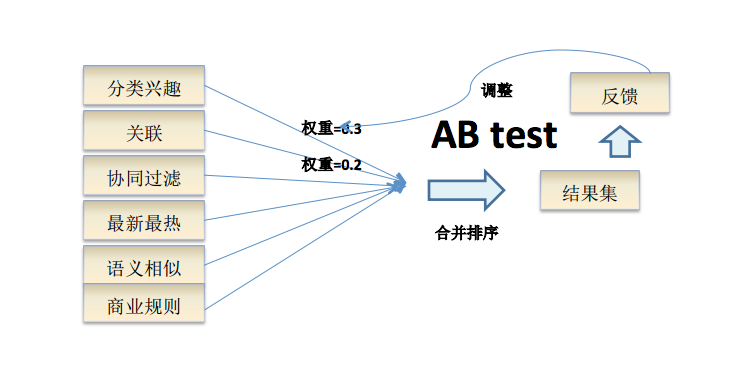
\includegraphics[scale=0.4]{figures/hl_abtest}}
      \figcaption{abtest调整标签权重}
      \label{pic:hl_abtest}
    \end{figure}

    \section{用户画像建模方式}
    根据用户在建模过程中的参与程度,用户兴趣建模可以分为用户手工定制建模、示例用户建模和自动用户建模。其中自动用户建模算法如\autoref{alg:init_userProfile}所示。
    \IncMargin{1em}
    \begin{algorithm}
      \SetKwData{Left}{left}\SetKwData{This}{this}\SetKwData{Up}{up}
      \SetKwFunction{Union}{Union}\SetKwFunction{FindCompress}{FindCompress}
      \SetKwInOut{Input}{input}\SetKwInOut{Output}{output}
      \Input{结构化用户注册信息和用户浏览行为}
      \Output{初始用户兴趣模型}
      \BlankLine
        从用户购买行为和反馈表单中提取兴趣标签及其对应的权重\\
        生成显式兴趣标签表,如{"动漫":"0.8","汽车":"0.4","美少女":"0.9"...}\\
        根据用户浏览行为获取用户兴趣标签获得隐式权重\\
        生成隐式兴趣标签表,如{"免费":"0.8","特价":"0.4","热门":"0.9"...}\\
        合并显式兴趣向量和隐式兴趣向量到当前用户画像\\
        如有新数据,返回第一步,否则跳出循环。
    \caption{k means}\label{alg:init_userProfile}
    \end{algorithm}
    \DecMargin{1em}

    \begin{itemize}
    \item 用户手工定制建模。指用户画像由用户自己手工输入或选择的用户建模方法,如用户手工输入感兴趣信息的关键词列表,或者是选择感兴趣的栏目等。在手机主题市场早期,用户手工定制建模是用户建模的主要方法。用户手工定制建模方法实现简单、效果也不错,但它存在以下三个方面问题:(1)完全依赖于用户,容易降低用户使用系统的积极性。(2)即使用户乐意手工输入用户画像,用户也难以全面,准确的罗列自己感兴趣的栏目或关键词,导致用户标签的质量有好有坏。(3)当用户兴趣发生变化时,用户必须重新输入用户画像,这给用户带来了额外的负担。
    \item 示例用户建模。指由用户提供与自己兴趣相关的示例及其类别属性来建立用户画像的建模方法。由于用户对自己的兴趣和偏好等最有发言权,因而用户提供的有关自己兴趣的示例最能集中、准确地反映用户的兴趣和偏好等特点。示例一般通过要求用户在浏览过程中标注自己的兴趣兴趣度,如喜欢、赞、踩和收藏等。
    \item 自动用户建模.指根据用户的浏览内容和浏览行为自动构建用户画像,自动用户建模由于无需用户主动提供信息,不会显示干扰用户,有利于提高个性化服务系统的亲和度,因此,自动建模技术当前用户画像领域热门研究方向。
    \end{itemize}

    \section{用户画像的维度分析}
    一个用户可以从多个方面去刻画,也就是说用户画像可以从多个维度来考虑和构建。作为虚拟电子商品交易平台,手机主题市场的用户在平台上通过某些行为(点击、浏览、购买)生产或获取信息,也通过其它一些行为(如转发、评论、赞)将信息传播出去,信息的传播是通过用户之间的社交关系所进行的,并且在生产、消费、传播信息的过程中对信息的选择和过滤体现了用户在兴趣方面的倾向性。由此,我们可以将用户画像按照\autoref{pic:hl_userDimension}所示的四个维度进行划分,即属性维度、兴趣维度、社交维度和行为维度。用户属性和用户兴趣是传统用户画像中包含的两个维度。前者刻画用户的静态属性特征,例如用户的身份信息(性别、年龄、受教育程度、学校等),后者则用于刻画用户在信息筛选方面的倾向(例如用户的购买能力、兴趣标签、能力标签等)。社交维度是从社交关系及信息传播的角度来刻画用户的。在社区中用户不在仅仅是一个个体,用户和用户之间的社交关系构成了一张网络,信息在这张网络中高速流动,但是这种流动并不是无差别的,信息的起始点,所经历的关键节点以及这些节点构成的关系圈都是影响信息流动的重要因素。行为维度是一个比较新的研究方向,目的是发现影响用户属性、信息变化的行为因素,分析典型用户群体的行为模式。一方面可以通过行为模式的复用来促进用户在手机主题应用平台的成长;另一方面也有利于平台认识用户,和发现新的或异常的用户行为。    
    \begin{figure}
    \centering
      \framebox{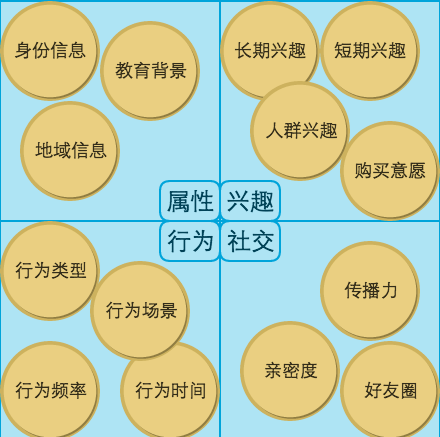
\includegraphics[scale=0.6]{figures/hl_userDimension}}
      \figcaption{用户画像维度划分}
      \label{pic:hl_userDimension}
    \end{figure}

        \subsection{属性维度}
        属性维度属于传统用户画像的范畴,即对用户的信息进行标签化。一方面,标签化是对用户信息进行结构化,方便计算机的识别和处理;另一方面,标签本身也具有准确性和非二义性,也有利于人工的整理、分析和统计。用户属性指相对静态和稳定的人口属性,例如:性别、年龄区间、地域、受教育程度、学校、公司等信息的收集和建立主要依靠产品本身的引导、调查、第三方提供等,在此基础上需要进行补充和交叉验证。
        \begin{itemize}
        \item 标签来源:不是所有的词都适合充当用户标签,这些词本身应该具有区分性和非二义性;此外,还需要考虑来源的全面性,除了用户主动提供的兴趣标签外,用户在使用的过程中的行为,构建的用户关系等也能够反应用户的兴趣,因此也要将其考虑在内。
        \item 权重计算:得到了用户的兴趣标签,还需要针对用户给这些标签进行权重赋值,用来区分不同标签对于该用户的重要程度。
        \end{itemize}

        \subsection{兴趣维度}
        由于用户兴趣维度的重要性,因此有一个独立于用户画像模块的兴趣探索模块,下一章节将会详细介绍到。用户兴趣是更加动态和易变化的特征,首先兴趣受到人群、环境、热点事件、行业等方面的影响,一旦这些因素发生变化,用户的兴趣容易产生迁移;其次,用户的行为多样且碎片化,不同行为反映出来的兴趣差异较大,在用户画像建模的过程中,主要考虑如下几个方面:
        \begin{itemize}
        \item 时效性:随着时间的变化,用户的兴趣会发生转移,有些兴趣会贯穿用户使用社交媒体的全过程,而有些兴趣则是受热点时间、环境因素等的影响。
        \item 长尾性:对于电商领域来讲,那些冷门的用户兴趣的总和可以和那些为数不多的大众化兴趣所占的市场份额相匹配或胜出。
        \item 兴趣和购买意愿的区分:用户具有某方面的兴趣,只代表了他愿意接受这方面的信息,并不能代表他具有购买相关内容的意愿。例如对于一些只看不买的用户,我们认为其购买意愿很小,因此对其会尽可能多的展示免费主题。
        \end{itemize}

        \subsection{社交维度}
        如果将主题应用平台的用户视作节点,用户之间的关系视作节点之间的边,那么这些节点和边将构成一个社交的网络拓扑结构,或称作社交图谱。消费信息就是在这个图谱上进行传播。从社交的维度建立用户画像,需要从不同的角度细致和全面地描述这个消费图谱的特征,反应影响信息传播的各层面上的因素,寻找节点之间的关联度,以及刻画图谱本身的结构特征。其中包括:
        \begin{itemize}
        \item 用户个体对消费信息传播的影响:不同用户在信息传播过程中的重要性不一样,影响大的用户对于信息的传播较影响小的用户更具有促进作用。
        \item 量化用户关系紧密度:存在社交关联的用户,关系越近的用户之间越容易产生相同的消费行为。
        \item 寻找相似的用户:消费中非对等的关系本身可以认为是一种认证,用户基于兴趣、消费态度等原因反应到线上的一种关联。那么在消费维度上的相似用户至少能反应他们在某种因素上的一致性。
        \item 识别关系圈:从关系图谱的本身的结构出发,从中发掘关联紧密的群体,有助于促销广告的精准投放和主题包的推广。以上关于关系建模的任务可以看作是逐步深入的,从“个体”-->“关联”-->“相似”-->“群体”的逐渐深入。
        \end{itemize}

        \subsection{行为维度}
        分析用户的行为,建立行为模式有两个任务:针对典型个体行为进行时序分片,分析用户成长的相关因素;针对典型群体的行为进行统计,为其构建通用的用户画像。
        \begin{itemize}
        \item 典型个体的行为时序分析。所谓典型个体是指某段时间内,成长比较突出的用户。例如从一个新用户从新注册到点击过百、浏览过千需要有一个积累过程,有些用户积累较快,有些较慢,而这些积累较快的用户可以作为典型个体;或者某些用户在某一阶段消费有限,但在某时刻消费激增,无论是消费金额还是数量都变化很大,这种也可以作为典型个体。针对典型个体,需要挖掘与其用户成长相关的行为因素。基本方法是对时间进行分片,获取用户在不同时间片上的行为统计,以及在各个时间分片上的用户成长指标(点击量、购买量、点击转换比等)。在此基础上针对用户行为的统计量的变化,利用关联性分析或回归来分析用户成长与哪些因素有关。
        \item 典型群体行为模式分析。针对典型个体,从用户的基本信息、人口信息、兴趣维度,可以将相似的典型用户划分为同一的群体,称作典型群体,针对典型群体中的用户按照成长程度进行划分,按不同的成长阶段统计用户行为,即建立了该典型群体的行为模型。例如,对于“年龄在20~30岁,女性,付费用户”这样的典型群体,从日点击量、月消费额等维度将其划分到初创、成长、快速提升、成熟等阶段,针对不同成长阶段内的行为组合进行统计,结果构成该群体的行为模式。如\autoref{pic:hl_usergroup}
        \end{itemize}

        \begin{figure}
        \centering
          \framebox{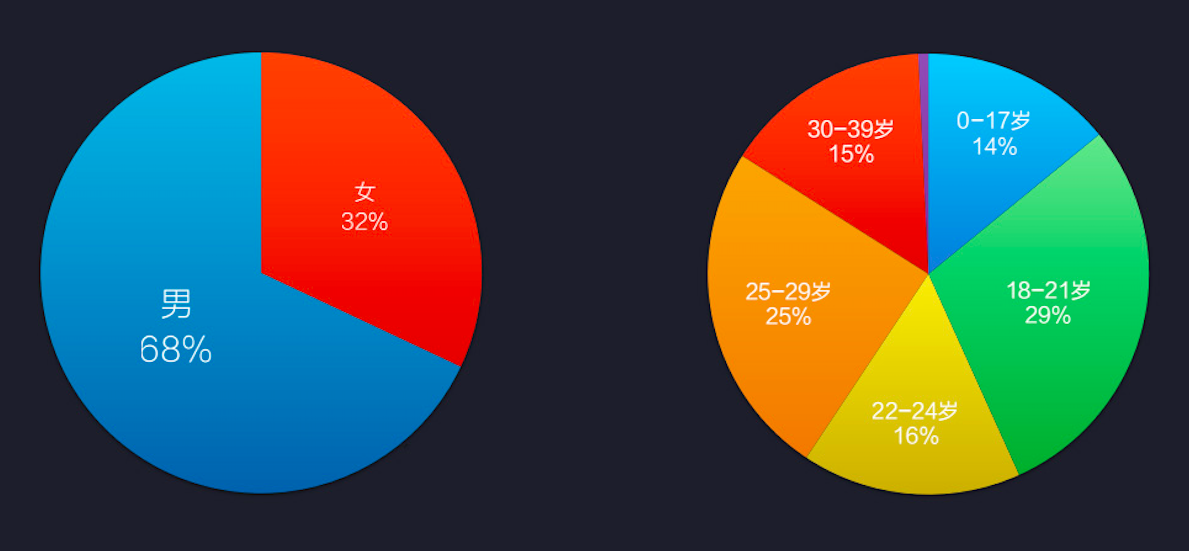
\includegraphics[scale=0.35]{figures/hl_usergroup}}
          \figcaption{手机主题市场用户群体分布}
          \label{pic:hl_usergroup}
        \end{figure}


    \section{用户画像应用场景}
      \subsection{优化手机主题市场供求}
      改变了原有的先设计、再销售的传统模式。第三方主题设计师在设计一款新产品前,会先设定好主题类型,然后通过用户画像平台中分析该用户群体的偏好,有针对性的设计产品,从而改变原先新产品高失败率的窘境,增强销售表现。如设计一款智能手表主题,面向28-35岁的年轻男性,通过在平台中进行分析,发现属性=“金属”、风格=“硬朗”、颜色=“黑色”/"深灰色"、价格区间=“中等”的偏好比重最大,那么就给新产品的设计提供了非常客观有效的决策依据。
      \subsection{提高新人留存率}
      工商管理有一个理论叫做,维护一个老用户的成本是获取新用户成本的五分之一甚至更低。所以如果能够把一些已经流失的用户召回来,这时候成本比拉一个新用户低得多,你做的事也会带来更大的价值。鉴于此公司启动了一个项目叫"用户画像之拉新",首先利用用户画像得出最近一个月没有登录过的用户数据,然后根据浏览时长分档,这是因为用户需要花自己的时间成本才能留下的最有价值的标签,之后利用用户静态标签,像姓名、职业、年龄、地域分布做进一步的细分,最后针对不同类型的用户提供不同的优惠活动。ABtest显示,与传统一刀切的推荐相比,基于用户画像的拉新留存率提高了约50\%。
      \subsection{用户消费等级分群}
      大至用户终端品牌、机型、操作系统,细至屏幕分辨率、屏幕尺寸,用户画像记录了每一个用户群体的详细终端特征。哪一类人群最容易被这款应用吸引,愿意为这款应用付费?开发者经常考虑的问题可以从用户画像找到答案。每一个用户群的价格分布、增值业务费用分布以及流量费用,包括用户详细的消费特征,比如付费频率,丰富了推荐系统的数据依据。
      \subsection{用户流失预警}
      一般情况用户在消费过程中会经历对如下几个期间:新鲜期,沉迷期,消退期,离开四个阶段,如何能够延长用户在应用的停留周期是需要解决的问题之一。用户画像可以辅助推荐系统进行流失用户特征分析,通过决策数算法,分析流失用户特征,建立不同原因流失的用户模型,然后通过这些特征得到当前在应用活跃用户中匹配流失概率高的用户数据。
      \subsection{反作弊}
      用户画像会对用户的消费能力、空闲时间、信用评级等维度进行打分;利用反作弊模型通过业务方访问收集数据,供安全部门参考。
    \section{总结}
      用户画像对于推荐系统来讲,主要如下几个方面的提升:提升推荐系统的精度,用户画像将用户的长期偏好融入到了推荐内容中,维护了推荐系统一致性。abtest显示,融合了用户画像的推荐模型比单纯的推荐模型在点击转化率指标提高了约2.8\%,考虑到300万用户的基数,2.8\%的提升是一个很大的进步;用户画像还解决新用户的冷启动问题,对于一个新注册用户来讲,推荐系统可以利用用户画像的静态信息,然后结合商品信息进行推荐;提高推荐系统的时效性,对用户行为的离线预处理,可以节约推荐系统的大部分计算时间。但是因为用户画像存储的数据都是历史数据,所以其不能实时准确的反映用户兴趣的变化,为了解决这个问题,我们引入了用户兴趣探索模块,将在下一章节件详细介绍。
